\documentclass[mathsans]{beamer}
%\documentclass[handout]{beamer}
% impression: handout, mais à supprimer pour projection
% si on veut avoir les overlays
\uselanguage{French}
\languagepath{French}
\usepackage[francais]{babel}
\usepackage{eurosym}
\usepackage[utf8]{inputenc}
\usepackage[T1]{fontenc}
\usepackage{url,movie15}
\usepackage{amsthm,amssymb,amsmath,algorithmic}
\usepackage{algorithmic}
\usepackage{listings}
\usepackage{tikz}
\usetikzlibrary{arrows,shapes}
\usetikzlibrary{positioning}
\usetikzlibrary{patterns}
\setbeamertemplate{theorems}[numbered]
\newcommand{\Xcut}{X_{\mbox{\scriptsize cut}}}
\newcommand{\xcut}{x_{\mbox{\scriptsize cut}}}
\newtheorem{consequence}{Consequence}
\renewcommand{\algorithmiccomment}[1]{//#1}
\newcommand{\RN}{\mbox{\,RN\,}}
\newcommand{\RU}{\mbox{\,RU\,}}
\newcommand{\RD}{\mbox{\,RD\,}}
\newcommand{\RZ}{\mbox{\,RZ\,}}
\newcommand{\ulp}{\mbox{\,ulp\,}}
\usepackage{hyperref}               %for hyperlinking and other
\newtheorem{algorithm}{Algorithm}
\newtheorem{observation}{Observation}
\newtheorem{property}{Property}
\newcommand{\ru}{{\bf u}}
\newtheorem{Cprogram}{C~Program}
\newcommand{\emin}{{e_{\mbox{\tiny min}}}}
\newcommand{\emax}{{e_{\mbox{\tiny max}}}}
\newcommand{\crlibm}{CRLibm}
\newcommand{\oguil}{\raisebox{0.3ex}{\tiny $\ll$}}
\newcommand{\fguil}{\raisebox{0.3ex}{\tiny $\gg$}}
\newcommand{\round}{\mathop{\circ}\nolimits}
\usetheme[secheader]{Boadilla}
\useinnertheme{rounded}
%\usetheme{Rochester}
\setbeamertemplate{footline}{
  \leavevmode%
  \hbox{%
  \begin{beamercolorbox}[wd=.3\paperwidth,ht=2.25ex,dp=1ex,center]{author in head/foot}%
    \usebeamerfont{author in head/foot}\insertshortauthor~~%(\insertshortinstitute)
  \end{beamercolorbox}%
  \begin{beamercolorbox}[wd=.4\paperwidth,ht=2.25ex,dp=1ex,center]{title in head/foot}%
    \usebeamerfont{title in head/foot}\insertshorttitle
  \end{beamercolorbox}%
  \begin{beamercolorbox}[wd=.3\paperwidth,ht=2.25ex,dp=1ex,right]{date in head/foot}%
    \usebeamerfont{date in head/foot}\insertshortdate{}\hspace*{2em}
    \insertframenumber{} / \inserttotalframenumber\hspace*{2ex} 
  \end{beamercolorbox}}%
  \vskip0pt%
}
\setbeamertemplate{theorems}[numbered]



\title[\'Equipe AriC]{\small{Améliorer le \alert{calcul}, en termes de \alert{performance, d'efficacité} et de \alert{fiabilité.}}}

\author[\'Evaluation LIP]{{\footnotesize\url{http://www.ens-lyon.fr/LIP/AriC/}}}
\institute[]{}
\date[Novembre 2014]{Novembre 2014 -- \'Evaluation du LIP}
\begin{document}


\begin{frame}[fragile]
\frametitle{AriC: Arithmetic and Computing}

\begin{minipage}{4.2cm}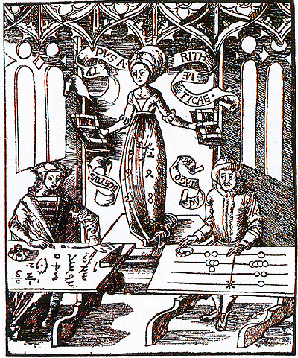
\includegraphics[width=4cm]{Figures/DameArithmetique.PDF}\end{minipage}
\begin{minipage}{6.3cm} \titlepage \end{minipage}~\\[0.51cm]
 \centerline{ \includegraphics[width=0.8cm]{Figures/LogoCNRS.pdf}\hspace{1cm} \includegraphics[width=2.0cm]{Figures/logoENS.jpg}\hspace{1cm}\includegraphics[width=2cm]{Figures/LogoINRIA.pdf}\hspace{1cm}\includegraphics[width=1.7cm]{Figures/logo_ucbl.jpg} }
\end{frame}

\begin{frame}
\frametitle{AriC: Arithmetic and Computing}
Améliorer le \alert{calcul}, en termes de \alert{performance, d'efficacité} et de \alert{fiabilité.}
\break
\begin{center}
\begin{tikzpicture}[scale=0.1]
\fill[red!05] (0,1) ellipse (20 and 12);
\draw[red!80, line width = 2] (0,1) ellipse (20 and 12);
\draw(0,2) node{Symbolique};
\fill[green!05] (50,1) ellipse (20 and 12);
\draw[green!80, line width = 2] (50,1) ellipse (20 and 12);
\draw(50,2) node{Numérique};
\draw[very thick,<->] (20,1) -- (30,1);
\fill[blue!05] (25,-25) ellipse (20 and 12);
\draw[blue!80, line width = 2] (25,-25) ellipse (20 and 12);
\draw(25,-25) node{Matériel};
\draw[very thick,<->] (10,-10) -- (12,-15);
\draw[very thick,<->] (39,-16) -- (42,-10);
\end{tikzpicture}
\end{center}

\end{frame}


\begin{frame}
\frametitle{AriC: Arithmetic and Computing}
%Améliorer le \alert{calcul}, en termes de \alert{performance, d'efficacité} et de \alert{fiabilité.}

\begin{itemize}
    \item algorithmes arithmétiques $\&$ leur implantation (matérielle, logicielle): \\
  \begin{minipage}{7cm}  
    \begin{itemize}
         \item arithmétique entière et virgule flottante;
         \item arithmétique complexe, multi-précision;
      \end{itemize} \end{minipage}~~
      \begin{minipage}{3cm}
      \includegraphics[width=2.9cm]{Figures/archisin.pdf}
      \end{minipage}
    \item méthodes d'approximation: \\
    \begin{minipage}{6.9cm}
      \begin{itemize}
            \item approximation sous contraintes particulières; 
            \item approximation certifiée;
       \end{itemize}
         \end{minipage}~~~~
      \begin{minipage}{3cm}
      \includegraphics[width=2.5cm]{Figures/mezzarobba-arith.pdf}
       \end{minipage}
    \item  réseaux euclidiens et cryptographie:\\[-0.2cm]
    \begin{minipage}{6.9cm}
       \begin{itemize}
            \item algorithmique des réseaux;
            \item cryptographie reposant sur les réseaux;
        \end{itemize}
      \end{minipage}~~~~
      \begin{minipage}{3cm}
      \includegraphics[width=1.6cm]{Figures/Resau.jpg}
      \end{minipage}
    \item calcul certifié et calcul formel:
    \begin{itemize}
       \item algèbre linéaire, systèmes polynomiaux, équations différentielles;
       \item arithmétique d'intervalles.
    \end{itemize}
 \end{itemize}
\end{frame}

\begin{frame}
\frametitle{AriC: Arithmetic and Computing}
%Améliorer le \alert{calcul}, en termes de \alert{performance, d'efficacité} et de \alert{fiabilité.}
%Équipe commune CNRS, ENS de Lyon, Inria et Université Claude Bernard Lyon 1.
Équipe commune\\[-0.65cm] \hspace{3cm}{ \includegraphics[width=0.7cm]{Figures/LogoCNRS.pdf}\hspace{0.5cm} \includegraphics[width=1.9cm]{Figures/logoENS.jpg}\hspace{0.5cm}\includegraphics[width=1.9cm]{Figures/LogoINRIA.pdf}\hspace{0.5cm}\includegraphics[width=1.2cm]{Figures/logo_ucbl.jpg} }\\[0.5cm]
\begin{itemize}
    \item fait suite à l'équipe Arénaire;
    \item Effectifs actuels:
    \begin{itemize}
          \item \alert{13 permanents:} 4 enseignants-chercheurs (3PR+1MCF), 7 chercheurs (3DR+4CR), 1 IR, 1 administratif;
         \item \alert{8 non-permanents:} 6 doctorants, 1 délégation, 1 postdoc;
      \end{itemize}   
    \item direction:
    \begin{itemize}
          \item $\longrightarrow$  30 juin 2013: Florent de Dinechin (maintenant PR INSA Lyon);
          \item juillet 2013 $\longrightarrow$ mars 2015: Jean-Michel Muller;
          \item mars 2015 $\longrightarrow$: Bruno Salvy et Gilles Villard.
     \end{itemize}
\end{itemize}
\end{frame}




\begin{frame}
\frametitle{Membres permanents présents actuellement}
\begin{small}
\begin{minipage}{6.2cm}
\alert{4 Enseignants-chercheurs}
\begin{itemize}
    \item Guillaume Hanrot, PR ENS Lyon;
    \item Fabien Laguillaumie, PR UCBL;
    \item Nicolas Louvet, MCF UCBL;
    \item Damien Stehlé, PR ENS Lyon;
 \end{itemize} 
 \alert{2 Ingénieurs et administratifs}
 \begin{itemize}
     \item Damien Séon, assistant, ENS Lyon;
     \item Serge Torres, IR ENS Lyon;
   \end{itemize}
\end{minipage}~
\begin{minipage}{6cm}
 \alert{7 Chercheurs}
 \begin{itemize}
    \item Nicolas Brisebarre, CR CNRS;
    \item Claude-Pierre Jeannerod, CR Inria;
    \item Vincent Lefèvre, CR Inria;
    \item Jean-Michel Muller, DR CNRS;
    \item Nathalie Revol, CR Inria;
    \item Bruno Salvy, DR Inria;
    \item Gilles Villard, DR CNRS.
 \end{itemize}
%\vspace{0.3cm}
\end{minipage}~\\[0.7cm]
\hrule~\\
\alert{Arrivées:} Hanrot, Laguillaumie, Salvy.\hspace{1cm}\alert{Départ:} de Dinechin.
\end{small}
\end{frame}


\begin{frame}
\frametitle{Membres non permanents présents actuellement}
\begin{small}
\begin{minipage}{6cm}
\alert{7 Doctorants}
\begin{itemize}
\item Silviu Filip (allocation ordinaire);
\item Sébastien Maulat (ENS Lyon);
\item Vincent Neiger (ENS Lyon);
\item Marie Paindavoine (CIFRE Orange Labs);
\item Antoine Plet (ENS Lyon);
\end{itemize}
\end{minipage}~
\begin{minipage}{6cm}
\begin{itemize}
\item Valentina Popescu (allocation Région Rhône-Alpes);
\item Serge Torres (ENS Lyon);
\end{itemize}

\alert{2 Autres}
\begin{itemize}
    \item Clément Pernet, MCF Grenoble 1, délégation CNRS puis Inria; 
    \item Benoît Libert, Chercheur CDD PALSE;
\end{itemize}
\end{minipage}
\end{small}
\end{frame}


%\begin{frame}
%\frametitle{Anciens doctorants}
%\begin{footnotesize}
%\begin{minipage}{6.1cm}
%\begin{itemize}
%\item Nicolas Brunie (CIFRE), soutenance 05/14 $\to$ Ingénieur Kalray Grenoble;
%\item Sylvain Chevillard (ENS Lyon), soutenance 07/09 $\to$ CR Inria Sophia;
%\item Mioara Jolde\c{s} (alloc. Région RA), soutenance 09/11 $\to$ CR CNRS Toulouse;
%\item Jingyan Jourdan-Lu (CIFRE), soutenance 11/12 $\to$ postdoc Inria Grenoble;
%\item Adeline Langlois (ENS Cachan), soutenance 10/14  $\to$ postdoc EPFL;
%\item \'Erik Martin-Dorel (alloc. ordinaire), soutenance 09/12 $\to$ MCF Toulouse;
%\item Ivan Morel (ENS Lyon), jusqu'à 08/11 $\to$ professeur de lycée;
%\item Christophe Mouilleron, soutenance 11/11 $\to$ professeur agrégé ENSIEE Evry;
%\end{itemize}
%\end{minipage}~
%\begin{minipage}{6.2cm}
%\begin{itemize}
%\item Hong-Diep Nguyen (Inria Cordi-S), soutenance 01/11 $\to$ postdoc U. Berkeley;
%\item Adrien Panhaleux (ENS Lyon), soutenance 08/12 $\to$ auto-entrepreneur;
%\item Bogdan Pasca (alloc. ordinaire), soutenance 09/11 $\to$ Altera, UK;
%\item David Pfannholzer (bourse MEFI), jusqu'à 10/11 $\to$ ingénieur Ingenieurbüro R. Sellger, Allemagne;
%\item Xavier Pujol (ENS Lyon), jusqu'à 08/12 $\to$ Google Zurich;
%\item Guillaume Révy (alloc. ordinaire), soutenance 12/09 $\to$ MCF Perpignan;
%\item Philippe Théveny (alloc. ordinaire), soutenance 10/14 $\to$ postdoc U. Denver;
%\end{itemize}
%\end{minipage}
%\end{footnotesize}
%\end{frame}
%
%\begin{frame}
%\frametitle{Anciens membres hors doctorants}
%\begin{small}
%\begin{minipage}{6.1cm}
%\alert{Enseignants-chercheurs}
%\begin{itemize}
%    \item Florent de Dinechin, MCF ENS Lyon (jusqu'à sept. 2013) $\to$ PR INSA Lyon;
% \end{itemize}
%\alert{Postdocs et ATER}
%\begin{itemize}
%    \item Rishiraj Bhattacharyya (06/12 -- 04/14);
%    \item Jingwei Chen (06/12 -- 12/12);
%    \item Sylvain Collange (10/10 -- 09/11);
%    \item Nicolas Estibals (09/12 -- 08/13);
%    \item Eleonora Guerrini (09/11 -- 08/12);
%    \item Marc Mezzarobba (12/11 -- 04/13);
%\end{itemize}
%\end{minipage}~
%\begin{minipage}{6.1cm}
%  \begin{itemize}
%    \item Andrew Novocin (09/09 -- 08/11);
%    \item Ioana Pasca (12/10 -- 12/12).
%   \end{itemize}
%\alert{Délégations}
%\begin{itemize}
%    \item Laurent-Stéphane Didier (09/11 -- 09/12), MCF Paris 6 en CRCT $\to$ PR Univ. Toulon;
%    \item Stef Graillat (09/13 -- 08/14), MCF Paris 6 en délégation CNRS $\to$ PR Paris 6;
%    \item Micaela Mayero (09/09 -- 08/10 puis 09/11 -- 08/12), MCF Paris 13 en délégation Inria;
%\end{itemize}
%%\vspace{1.6cm}
%\end{minipage}
%\end{small}
%\end{frame}

\begin{frame}
\frametitle{Quelques faits marquants}
\begin{itemize}
\item \alert{Médaille de bronze du CNRS} attribuée à Damien Stehlé en 2012;
\item \alert{Médaille d'argent du CNRS} attribuée à Jean-Michel Muller en 2013;
\item \alert{ERC Starting Grant} attribuée en 2013 à Damien Stehlé pour son projet \emph{Lattices: Algorithms and Cryptography (LattAC)};
\item \alert{Prix La Recherche 2013} pour les Sciences de l'Information attribué à Vincent Lefèvre, Nicolas Louvet,  Jean-Michel Muller et notre collègue danois Peter Kornerup;
\item \alert{IEEE Working Group P1788 for standardization of interval arithmetic,} présidé par Nathalie Revol;%. Se termine en 2015;
\end{itemize}~\\[-1cm]
\begin{minipage}{9.5cm}
\begin{itemize}
\item \alert{Handbook of Floating-Point Arithmetic} (Birkhäuser 2010; 572 pages);
\end{itemize}
\end{minipage}
\begin{minipage}{2cm}
\includegraphics[scale=1.2]{Figures/handbook-fpa.jpg}
\end{minipage}

\end{frame}


%\begin{frame}
%\frametitle{Quelques faits marquants (suite)}
%\begin{itemize}
%
%\item \alert{Collaborations actives} avec STMicroelectronics, Kalray, et Orange Labs: contrats, projets communs, publications communes, 2 CIFRE\ldots
%\item \alert{Production logicielle:} CRlibm, FLIP, FloPoCo, fplll, Sollya, etc.;
%\item Organisation à l'ENS  Lyon de   \alert{SCAN 2010} 
%(Scientific Computing, Computer Arithmetic, and Validated Numerics): 120 participants de 20 nationalités;
%%\item ISSAC 2013 Best student paper awarded to Pierre Lairez. 
%\end{itemize}
%\end{frame}

\begin{frame}
\frametitle{Quelques résultats — Réseaux et Cryptographie}
\vspace*{0.5cm}

\hspace*{-0.2cm}

\begin{small}
\begin{tikzpicture}[scale=0.13]

%%% LWE

\fill[red!05] (0,1) ellipse (20 and 12);
\draw[red!80, line width = 2] (0,1) ellipse (20 and 12);
\draw (0,4.8) node[red,scale=0.8] {Learning With Errors};
\draw (4,6.8) node[red, scale=0.6] {dimension $n$, modulo $q$};
\draw (3,-5) node[scale=0.5]  {\colorbox{blue!30}{$\mathbf{A}$}
$\leftarrow \text{uniforme dans }\mathbb{Z}_q^{m \times n}$};
\draw (2.5,-6.7) node[scale=0.5]  {\colorbox{green!30}{$\mathbf{s}$}
$\leftarrow \text{uniforme dans } \mathbb{Z}_q^{n}$};
\draw (2.5,-8) node[scale=0.5]  { \colorbox{red!80}{$e$} est une petite erreur};
\draw (10,-3) node[red,scale=0.5]  { $ \mathbf{ m \geq n }$ };
\draw (40,1) node[red,scale=0.7]{Preuve de la difficulté classique de LWE};
\draw (40,-1) node[red,scale=0.7]{ pour tout module (STOC 2013)};

\draw (-10,-4) node[red,scale=0.7] {et/ou};
\draw (-10,-6) node[red,scale=0.8] {SIS};

\draw[thick] (-5.2,4) arc (155:205:8) ;
\draw[thick] (7,4) arc (25:-30:8) ;

\draw (-0.5,0.2) node[scale=0.8] {\textbf{,}};
\draw [->] (9,0.5) -- (11,0.5) node[scale=0.5] [midway, above] {trouver};
\fill[green!30] (12,0) rectangle (12.9,3) ;
\draw (12.2,0) -- (12.2,3) ;
\draw (12.2,0) -- (12.9,0) ;
\draw (12.2,3) -- (12.9,3) ;
\draw (12.9,0) -- (12.9,3) ;
\draw (12.45,1.5) node[scale=0.5] {$ \mathbf{s} $};

%\draw (-9.5,1) node[scale=0.6] {Given};

\fill[blue!30] (-4,-2) rectangle (-1,3) ;
\draw (-4,-2) -- (-4,3) ;
\draw (-1,-2) -- (-1,3) ;
\draw (-4,-2) -- (-1,-2) ;
\draw (-4,3) -- (-1,3) ;
\draw (-2.5,0.5) node[scale=1] {$\mathbf{A}$} ;

% Matrice 1
\fill[blue!30] (0,-2) rectangle (3,3) ;
\draw (0,-2) -- (0,3) ;
\draw (3,-2) -- (3,3) ;
\draw (0,-2) -- (3,-2) ;
\draw (0,3) -- (3,3) ;
\draw (1.5,0.5) node[scale=1] {$\mathbf{A}$} ;

% Vecteur 1
\fill[green!30] (3.5,0) rectangle (4.2,3) ;
\draw (3.5,0) -- (3.5,3) ;
\draw (3.5,0) -- (4.2,0) ;
\draw (3.5,3) -- (4.2,3) ;
\draw (4.2,0) -- (4.2,3) ;
\draw (3.85,1.5) node[scale=0.5] {$ \mathbf{s} $};

\draw (5,0.5) node[scale=0.6] {$\mathbf{+}$};

% Vecteur 2
\fill[red!80] (5.7,-2) rectangle (6.5,3) ;
\draw (5.7,-2) -- (5.7,3) ;
\draw (5.7,-2) -- (6.5,-2) ;
\draw (5.7,3) -- (6.5,3) ;
\draw (6.5,-2) -- (6.5,3) ;

\draw (6.15,0.5) node[scale=0.5] {$ \mathbf{e} $};

% dimension
\draw [<->] (-4.2,-2) -- (-4.2,3) node[scale=0.4] [near end, left] {$m$} ;
\draw [<->] (-4,-2.2) -- (-1,-2.2) node[scale=0.4] [midway, below] {$n$};

%%%%%%%%%%%%%%
% Réseaux



\fill[blue!03] (25,18) ellipse (14 and 9);
 \draw[blue!80,line width=2] (25,18) ellipse (14 and 9);

%\draw[blue] (35,18) node[scale=0.6] {worst-case};


\draw (25,24) node[blue,scale=1] {Réseau};
\draw (25,12) node[blue,scale=0.7] {$\rightarrow$  GapSVP};
%\draw (25,12) node[blue,scale=0.8] {in dimension $n$ large};

\draw (20,15) node[scale=0.6] {$\bullet$} ;
\draw (20,21) node[scale=0.6] {$\bullet$} ;
\draw (22,15) node[scale=0.6] {$\bullet$} ;
\draw (24,15) node[scale=0.6] {$\bullet$} ;
\draw (26,15) node[scale=0.6] {$\bullet$} ;
\draw (21,18) node[scale=0.6] {$\bullet$} ;
\draw (23,18) node[scale=0.6] {$\bullet$} ;
\draw (25,18) node[scale=0.6] {$\bullet$} ;
\draw (22,21) node[scale=0.6] {$\bullet$} ;
\draw (24,21) node[scale=0.6] {$\bullet$} ;
\draw (26,21) node[scale=0.6] {$\bullet$} ;
\draw (27,18) node[scale=0.6] {$\bullet$} ;
\draw (29,18) node[scale=0.6] {$\bullet$} ;
\draw (28,15) node[scale=0.6] {$\bullet$} ;
\draw (30,15) node[scale=0.6] {$\bullet$} ;
\draw (28,21) node[scale=0.6] {$\bullet$} ;
\draw (30,21) node[scale=0.6] {$\bullet$} ;

\draw[blue,->] (25,18) -- (27,18) node [midway, below, scale=0.6]
{$\mathbf{b}_1$};

\draw[blue] (25,18) circle(2);

\draw (56,20) node[blue,scale=0.7]{Première analyse en complexité };
\draw (56,18) node[blue,scale=0.7]{de l'algorithme BKZ (CRYPTO 2011)};

%%%%%%%%%%
% Alice et Bob

\fill[green!10] (27,-14.5)ellipse(12 and 8);
\draw[line width = 2,green] (27,-14.5)ellipse(12 and 8);

\fill[blue!60] (22,-15)ellipse(1.2 and 2.4) (22,-11)circle(1);
%\draw[blue!60, very thick] (22,-18.5) node[scale=1] {Alice};

\fill[red!40] (32,-15)ellipse(1.2 and 2.4) (32,-11)circle(1);
%\draw[MyGreen] (32,-18.5) node[scale=1] {Bob};

%\draw[MyGreen] (27,-19.5) node[scale=0.7] {Group Signature};

\draw[blue,thick,->] (25,-13) -- (29,-13);
\draw[red,thick, <-] (25,-14) -- (29,-14);

\draw[blue, thick,->] (25,-15.5) -- (29,-15.5);
\draw[red,thick, <-] (25,-16.5) -- (29,-16.5);


%%%%%%%%%%%%%%%%%%%%%%%%%%%%%%%

\draw (-9,23) node[scale=1.0] {1. Fondements};
\draw (-7,-18) node[scale=1.0] {2. Constructions};

\draw[line width = 2,->] (11.2,20) to[bend right] (0,13);
\draw[line width = 2,->] (0,-11) to[bend right] (15,-15.5);

\draw (43,-6) node[scale=0.7] {Chiffrement basé};
\draw (45,-8) node[scale=0.7] {sur LWE};


\draw (46,-13) node[scale=0.7] {Signature reposant};
\draw (47,-15) node[scale=0.7] { sur SIS};

\draw (45,-21) node[scale=0.7] {Signature de groupe};
\draw (47,-23) node[scale=0.7] {reposant sur SIS et LWE};

\draw (12,-24) node[green,scale=0.7]{Signatures de groupe plus efficaces };
\draw (12,-26) node[green,scale=0.7]{à base de réseaux euclidiens (Asiacrypt 2013)};

\end{tikzpicture}
\end{small}

\end{frame}

%\begin{frame}
%\frametitle{Quelques résultats — Réseaux et Cryptographie}
%\begin{itemize}
%    \item \textcolor{black}{D. Stehlé} et R. Steinfeld: preuve de sécurité du cryptosystème NTRU (Eurocrypt 2011);
%    \item \textcolor{black}{A. Novocin, D. Stehlé, G. Villard:} \alert{Réduction LLL de temps quasi-linéaire} (STOC 2011);
%    \item \textcolor{black}{G. Hanrot, X. Pujol et D. Stehlé:} Première analyse en complexité de l'algorithme \alert{BKZ}  (Crypto 2011);
%\end{itemize}
%\end{frame}

\begin{frame}
\frametitle{Quelques résultats — Arithmétique virgule flottante}
Algorithme de Kahan pour \alert{$x = ad-bc$} avec un \alert{FMA.}\\[0.5cm]
\begin{minipage}{4.0cm}
\definecolor{MyLightBlue}{rgb}{0.3, 0.6, .7}
\textcolor{MyLightBlue}{\begin{algorithmic}[0]
   \STATE{${\hat w} \gets \RN(bc)$}
   \STATE{$e \gets \RN({\hat w} - bc)$}
   \STATE{${\hat f} \gets \RN(ad-{\hat w})$}
   \STATE{${\hat x} \gets \RN({\hat f} + e)$}
   \STATE{Return $\hat{x}$}
\end{algorithmic}~\\[0.05cm]}
($\RN(t) =  t$ arrondi au nombre VF le + proche)\\[0.05cm]
\alert{
\[ u = 2^{-p}
\]} $p$: précision du système VF utilisé.
\end{minipage}~~~~~~~~
\begin{minipage}{7.5cm}

\begin{itemize}
   \item approche classique  (Higham, 2002): 
  \alert{ \[
   |{\hat x}-x| \le H \cdot{} |x|
   \]}
   avec $H = 2u+u^2 + (u+u^2) u\frac{|bc|}{|x|}$
   $\to$~précis tant que {$u|bc| \not\gg |x|$}
   \item en utilisant des propriétés de  $\RN$\footnote{Math. Comp., Oct. 2013}
  \alert{ \[|{\hat x}-x| \le 2u|x|\] } \alert{asymptotiquement optimal}
   \item[$\to$] $\times{}, \div{}$ complexes.
   \end{itemize}
\end{minipage}
\end{frame}


\begin{frame}
\frametitle{Quelques résultats — Approximations rigoureuses}
\begin{minipage}{4.5cm}
\includegraphics[width=4cm]{Figures/CourbeMioara.jpg}
\end{minipage}~~~
\begin{minipage}{4cm}
\[
J = \int_0^3 \sin \left( \frac{1}{\left(10^{-3} + (1-x)^2\right)^{3/2}} \right) dx
\]
\end{minipage}

\begin{minipage}{6cm}
\begin{itemize}
   \item Maple15: 0.7499743685;
   \item PARI/GP: 0.7927730971479080755;
   \item Mathematica, Chebfun: pas de réponse\ldots{}
   \item Chen, ’06: 0.7578918118
   \item \alert{$J =$ 0.749974368527 [1,3]}
\end{itemize}
\end{minipage}
\begin{minipage}{5.4cm}
\begin{itemize}
    \item thèse M. Joldes, 2011;
    \item {Chebyshev interpolation polynomial-based tools for rigorous computing}, ISSAC'10.
\end{itemize}
\begin{minipage}{1.8cm}
\includegraphics[width=1.5cm]{Figures/satellites.pdf}
\end{minipage}
\begin{minipage}{3.1cm}
\begin{tiny}
Collision de satellites (LAAS)
\end{tiny}
\end{minipage}
\end{minipage}
\end{frame}

\begin{frame}
\frametitle{Quelques résultats -- Complexité en calcul formel}

\begin{minipage}{9cm}
\begin{itemize}
\item \alert{Interpolation de polynômes multivariés} :
\begin{itemize}
\item Nouveaux algorithmes, à base d'algèbre linéaire structurée
\item Application : meilleurs coûts connus pour le décodage en liste des codes de Reed-Solomon
\end{itemize}
\item \alert{Équations différentielles linéaires:} algorithmes exacts plus rapides pour l'intégration;

\item \alert{Résolution de systèmes polynomiaux}: analyse de complexité des meilleurs algorithmes.{\footnotesize$^1$}
\end{itemize}
\hrule~\\
\begin{footnotesize}{$^1$J. of Symbolic Computation, 2014.}\end{footnotesize}
\end{minipage}
\begin{minipage}{2.5cm}
\includegraphics[width=2.5cm]{Figures/interpolation_neiger.pdf}\\[0.5cm]
\includegraphics[width=2.5cm]{Figures/tore-cycles.pdf}\\[0.5cm]
\includegraphics[width=2.5cm]{Figures/mat8.jpg}
\end{minipage}

\end{frame}

%\begin{frame}
%\begin{itemize}
%    \item A. Bostan, P. Lairez et \textcolor{black}{B. Salvy:} \alert{Creative telescoping for rational functions using the Griffiths-Dwork method}. \emph{Distinguished Student Award} d'ISSAC'13;
%    \item \textcolor{black}{N. Brunie, F. de Dinechin} et B. de Dinechin: brevet \alert{Mixed-Precision Merged Multiplication and Addition Operator}, 2012;
%\end{itemize}
%\end{frame}

\begin{frame}[fragile]
\frametitle{Devenir des doctorants de la période}
\def\angle{0}
\def\radius{2.4}
\def\cyclelist{{"lime","green","olive","pink","blue","red"}}
\newcount\cyclecount \cyclecount=-1
\newcount\ind \ind=-1
\begin{tikzpicture}[nodes = {font=\sffamily},scale=0.8]
  \foreach \percent/\name in {
      4/ CDI industrie,
      2/Chargés de Recherche (Inria et CNRS),
      2/Maîtres de Conférences,
      4/PostDoc,
      2/Agrégés,
      1/Autres,
    } {
      \ifx\percent\empty\else               % If \percent is empty, do nothing
        \global\advance\cyclecount by 1     % Advance cyclecount
        \global\advance\ind by 1            % Advance list index
    %    \ifnum3<\cyclecount                 % If cyclecount is larger than list
    %      \global\cyclecount=0              %   reset cyclecount and
     %     \global\ind=0                     %   reset list index
   %     \fi
        \pgfmathparse{\cyclelist[\the\ind]} % Get color from cycle list
        \edef\color{\pgfmathresult}         %   and store as \color
        % Draw angle and set labels
        \draw[fill={\color!50},draw={\color}] (0,0) -- (\angle:\radius)
          arc (\angle:\angle+\percent*24:\radius) -- cycle;
        \node at (\angle+0.5*\percent*24:0.7*\radius) {\percent\,};
        \node[pin=\angle+0.5*\percent*24:\name]
          at (\angle+0.5*\percent*24:\radius) {};
        \pgfmathparse{\angle+\percent*24}  % Advance angle
        \xdef\angle{\pgfmathresult}         %   and store in \angle
      \fi
    };
\end{tikzpicture}
\end{frame}

\begin{frame}
\frametitle{Production scientifique (hors logiciels)}
\begin{itemize}
   \item livre «Handbook of Floating-Point Arithmetic»;
   \item 41 articles dans des journaux internationaux;
   \item 7 conférences invitées;
   \item 84 communications à des conférences internationales;
   \item 2 brevets.
\end{itemize}
\end{frame}

\begin{frame}
\frametitle{Production logicielle}

Amélioration du calcul: de la preuve de faisabilité (CRLibm) aux applications industrielles (FLIP).
\begin{itemize}
\item \alert{CRLibm:} bibliothèque de fonctions élémentaires avec arrondi correct;
\item  \alert{FloPoCo:} générateur d'opérateurs arithmétiques pour FPGAs;
\item \alert{FLIP:} bibliothèque virgule flottante pour processeurs entiers;
\item \alert{FPLLL:} bibliothèque de réduction de réseaux euclidiens;
\item \alert{GFUN:} bibliothèque de calcul formel pour la D-finitude;
\item contribution à \alert{LinBox:} algèbre linéaire exacte;
\item  contribution à la bibliothèque \alert{GNU MPFR} (basée au Loria).
\end{itemize}
(peuvent être obtenus à \url{http://www.ens-lyon.fr/LIP/AriC/}).
\end{frame}

\begin{frame}
\frametitle{Implication dans des projets}
%\begin{minipage}{7.8cm}
\begin{itemize}
    \item Pilotage de trois projets ANR: \alert{EVA-Flo} (2006--2010,  N. Revol); \alert{TaMaDi} (2010--2013,  J.-M. Muller) et \alert{FastRelax} (2014--2018,  B. Salvy);
%    \end{itemize}
%\end{minipage}
%\begin{minipage}{4cm}~\\[-1cm]
% \includegraphics[width=3.0cm]{Figures/logoTaMaDi.pdf} 
%\end{minipage}
%\begin{itemize}
     \item participation aux projets \alert{TCHATER} (2008--2011), \alert{LAREDA} (2008--2011),  \alert{HPAC} (2011--2014), et \alert{MetaLibm} (2013--2017);
     \item D. Stehlé est porteur de \alert{l'ERC Starting Grant LattAC} (2013--2018);
    \item B. Libert est porteur du projet PALSE (Programme d'Avenir Lyon-St Etienne, 2014--2016) \alert{Towards practical enhanced asymmetric encryption schemes} (500 k\euro{} pour 2 ans).
\end{itemize}
\end{frame}

\begin{frame}
\frametitle{Animation scientifique}
\begin{itemize}
    \item \alert{direction d'unités:} %~~\includegraphics[width = 1cm]{Figures/logo_lip.pdf} ~~\includegraphics[width = 1cm]{Figures/logo-gdr-im.jpg}
    \begin{itemize}
         \item direction du LIP  
         \item co-direction du GDR IM  (+ responsabilité pôle et GT)
    \end{itemize}
    \item \alert{editorial boards:} Journal
 of Symbolic Computation, Journal of Algebra, IEEE Transactions on Computers;
   \item \alert{comités de programme et comités de pilotage:} ACM-CCS, Analco, ANTS, AofA, IEEE ARITH, IEEE ASAP, Asiacrypt, CRYPTO, Eurocrypt, FPL, FPT, Indocrypt, ISSAC, PASCO, PKC, SCAN;
   \item \alert{organisation d'événements:} SCAN 2010; \'Ecole de Printemps d'Informatique Théorique 2013; Journées Nationales du GDR IM 2013;  ARITH'2015;
   \item \alert{présidence} du comité de standardisation  IEEE P1788;
   \item \alert{conseils scientifiques:} INS2I, Cerfacs, ENS Lyon, ENSIIE \'Evry, Grenoble INP;
   \item \alert{doctorants:} conseil de labos et journée des doctorants.
\end{itemize}
\end{frame}

\begin{frame}
\frametitle{Participation à l'évaluation de la recherche}
\begin{itemize}
     \item vice-présidence de la Commission d'\'Evaluation Inria;
     \item présidence des comités d'évaluation Aeres du LIMOS (2011), du LIAFA (2012), de PPS (2012);
     \item participation aux comités  du GREYC (2010); du LIRMM (2013);
     \item vice-présidence du CES (Comité d'Evaluation Scientifique) «Mathématiques et Informatique Théorique» de l'ANR en 2014;
     \item jury de recrutement CR2 Inria GRA (2009, 2013 et 2014);
     \item 8 comités de sélection MCF;
     \item 6 comités de sélection PR;
     \item participation jury PES Inria (2013), présidence jury PES CNRS/INS2I (2014).
 \end{itemize}
\end{frame}



\begin{frame}
\frametitle{Enseignement et études doctorales}
\begin{itemize}
   \item \alert{direction du département d'informatique} de l'ENS Lyon;
   \item responsabilité du Master d'Informatique à l'ENS Lyon;
   \item responsabilité de la 2ème année «Ing\'enierie des Risques» du Master SAFIR (Lyon 1);
   \item forte implication dans des cours de Master à l'ENS Lyon et à l'ISFA (Univ. Lyon 1);
   \item participation au conseil de l'ED Infomaths.
\end{itemize}
\end{frame}

\begin{frame}
\frametitle{Relations industrielles}
\begin{itemize}
    \item Compilation Expertise Center de \alert{STMicroelectronics:  }
    \begin{itemize}
          \item Mediacom (Nano2012);
          \item CIFRE (Jourdan-Lu), 
          \item projet Région Rhône-Alpes, 
          \item Nano2017;
     \end{itemize}
    \item \alert{Kalray:} financement thèse Brunie;
    \item \alert{Orange Labs:} CIFRE (Paindavoine);
    \item \alert{Bosch:} conseil;
    \item donations \alert{Intel}, \alert{Altera} (carte d'accélération FPGA).
 \end{itemize}
\end{frame}

\begin{frame}
\frametitle{Diffusion, vulgarisation}
\begin{itemize}
   \item N. Revol: une vingtaine d'interventions en lycées (encourager aux carrières scientifiques) + journées «maths en jeans» + Forum des jeunes mathématicien-ne-s + \ldots{};
   \item N. Brisebarre: organisateur scientifique du cycle «Éclats de sciences», à la maison du livre, de l'image et du son de Villeurbanne. 3~conférences/an;
 \end{itemize}
 \begin{minipage}{4cm}
 \begin{itemize}
   \item 2 articles dans «La Recherche»: sept. 2013 (2 p.) et oct. 2014 (7 p.).
 \end{itemize}
\end{minipage}
 \begin{minipage}{7cm}
 \includegraphics[scale=0.08]{Figures/StehleLaRecherche.jpg}~~~~~\includegraphics[scale=0.19]{Figures/MullerLaRecherche.jpg}
 \end{minipage}
 \end{frame}

\begin{frame}
\frametitle{Projet de recherche}
\begin{center}
\begin{tikzpicture}[scale=0.1]
\fill[red!05] (0,1) ellipse (20 and 12);
\draw[red!80, line width = 2] (0,1) ellipse (20 and 12);
\draw(0,2) node{Symbolique};
\fill[green!05] (50,1) ellipse (20 and 12);
\draw[green!80, line width = 2] (50,1) ellipse (20 and 12);
\draw(50,2) node{Numérique};
\draw[very thick,<->] (20,1) -- (30,1);
%\fill[blue!05] (25,-25) ellipse (20 and 12);
%\draw[blue!80, line width = 2] (25,-25) ellipse (20 and 12);
%\draw(25,-25) node{Matériel};
%\draw[very thick,<->] (10,-10) -- (12,-15);
%\draw[very thick,<->] (40,-15) -- (42,-10);
\end{tikzpicture}
\end{center}

\alert{Trois volets:}
\begin{itemize}
     \item Réseaux euclidiens: algorithmes et cryptologie;
     \item Méthodes d'approximation efficaces;
     \item Noyaux de calcul fiables et haute performance.
 \end{itemize}
\end{frame}



\begin{frame}
\frametitle{Projet de recherche~--~1. Réseaux euclidiens: algorithmes et cryptologie}
         \begin{itemize}
               \item \alert{algorithmes sur les réseaux:} algorithmes rapides de réduction; compromis entre temps de calcul et taille de la base calculée; algorithmes de recherche du vecteur le plus court;
               \item \alert{cryptographie à base de réseaux:} renforcer les fondations; améliorer les performances des primitives; montrer que les réseaux permettent des primitives élaborées;
               \item \alert{applications:} équations diophantiennes, cryptanalyse de variantes de RSA.
          \end{itemize}
\end{frame}

\begin{frame}
\frametitle{Projet de recherche~--~2. Méthodes d'approximation efficaces}
           \begin{itemize}
                 \item \alert{calcul formel pour construction d'approximations certifiées:} approximations de solutions d'équations différentielles linéaires; automatisation $\to$ fonctions «rares», adaptation rapide à un nouveau contexte (exigences, processeur, etc.);
                 \item \alert{filtres certifiés,} méthodes optimales d'arrondi de coefficients;
                 \item \alert{dilemme du fabricant de tables:} optimisation/réécriture des algorithmes existants; techniques diophantiennes pour attaquer la quadruple précision.
           \end{itemize}
\end{frame}

\begin{frame}
\frametitle{Projet de recherche~--~3. Noyaux de calcul fiables et haute performance}
\begin{itemize}
     \item \alert{construction et analyse d'algorithmes symboliques ou numériques:}
         \begin{itemize}
             \item côté symbolique: jusqu'ici, algorithmes rapides pour matrices polynomiales et structurées, indépendamment. Exploiter les liens;
             \item côté numérique: nettoyer/revisiter des résultats classiques (bornes), estimation de conditionnements, comparaison de représentations en arithmétique d'intervalles (p.ex. mid-rad vs. bornes);
          \end{itemize}
     \item \alert{virgule flottante symbolique:} manipulation de nombres VF comme expressions en fonction de la base et de la précision;
     \item \alert{multi-précision haute performance:} précision d'au plus quelques centaines de bits.
\end{itemize}
\end{frame}

\begin{frame}
\frametitle{Conclusion}
\begin{minipage}{4.2cm}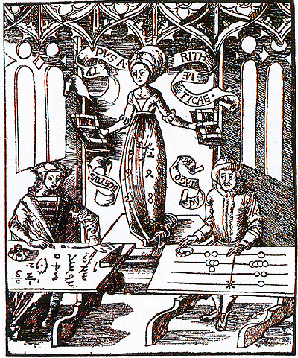
\includegraphics[width=4cm]{Figures/DameArithmetique.PDF}\end{minipage}
\begin{minipage}{7.5cm} 
\begin{itemize}
    \item \alert{grande équipe} (4 EC + 7 C + 2 ITA + 7 doc + 2 postdoc);
    \item spectre large, avec comme motto \alert{l'amélioration du calcul,} en termes de performance, d'efficacité et de fiabilité;
    \item de la \alert{théorie} aux \alert{applications industrielles;}
    \item vrai souci de \alert{diffusion;}
     \item forte implication des permanents dans \alert{l'animation scientifique} locale, nationale et internationale.

\end{itemize}
\end{minipage}
\end{frame}

\end{document}

